%%
%%      

\section*{What is Bacula-web?}
\label{_ChapterStart1}
\index[general]{Bacula-web!What is }
\index[general]{What is Bacula-web? }
\addcontentsline{toc}{section}{What is Bacula-web?}


Bacula-web is a php based web program that provides you a
summarized output of jobs that have already run. It obtains 
its information from your Bacula catalog database. Aside from a
nice graphical display, it provides summaries of your 
jobs, as well as graphs of job usage. This is a fairly high
level Bacula management tool.

\section*{Requirements}
\index[general]{Requirements}
\addcontentsline{toc}{section}{Requirements}

\begin{itemize}
\item You must have a web server
\item You must have PHP installed and working
      with your web server. We have tested 
      php versions 4.3.4 and 5.0.4.  For more information
      on php, please see:
      \elink{http://www.php.net}{http://www.php.net}.
\item The following packages should be installed
      or configured as part of PHP.
   \begin{itemize}
   \item Gettext (optional)
   \item GD 2.x or greater
   \item TrueType (optional)
   \item Pear DB (http://pear.php.net/package/DB)
   \item MySQL or PostgreSQL (SQLite is not supported)
   \item The dbsize contrib package if you use PostgreSQL
   \end{itemize}
\item Bacula must also be installed and working, but does not
      need to be running to use Bacula-web.
\item Your MySQL or PostgreSQL program must be running.
\end{itemize}

\section*{Installation}
\index[general]{Installation}
\addcontentsline{toc}{section}{Installation}

\begin{itemize}
\item Copy the bacula-web distribution to the root
   directory or a subdirectory of your web server root.
\item Edit {\bf configs/bacula.conf} and put your preferences
   as well as ensuring that the database configuration parameters
   point to the Bacula database you are using.
\item Make sure that {\bf short_open_tag} is turned on in your
   php.ini file.
\end{item}


\section*{Testing the Installation}
\index[general]{Testing the Installation}
\addcontentsline{toc}{section}{Testing the Installation}

\begin{itemize}
\item Run {\bf test.php} from your web browser.
   It should produce output that looks like:
\begin{verbatim}
Checking system for dependencies...

 Checking gettext:  YES   Language support enabled    
 Checking Pear(DB): YES   Pear DB enabled    
 Checking GD:       YES   GD support enabled    


 Please, click the link below to test your graph system capabilities
 (Bacula-web only use PNG): Test
\end{verbatim}

\item If gettext, Pear(DB) and GD all indicate yes, then things are going
   in the right direction. If not, you should correct each one before 
   proceeding.

\item If Pear(DB) is not installed and you have PHP 4.3.11 or newer, you
   can use the command:

\begin{verbatim}
pear install DB
\end{verbatim}
to install it.

After installing it, check by doing:

\begin{verbatim}
pear list
\end{verbatim}

On my machine (Kern), I get:
\begin{verbatim}
Installed packages:
===================
Package              Version State
Archive_Tar          1.1     stable
Console_Getopt       1.2     stable
DB                   1.7.6   stable
HTML_Template_IT     1.1     stable
HTTP                 1.3.5   stable
Mail                 1.1.4   stable
Net_SMTP             1.2.6   stable
Net_Socket           1.0.6   stable
Net_UserAgent_Detect 2.0.1   stable
PEAR                 1.3.5   stable
XML_Parser           1.2.6   stable
XML_RPC              1.4.0   stable
\end{verbatim}



\item When everything is installed, click on the {\bf Test} link at the
   bottom, which will bring up a new page with a number of PHPlot test graphs,
   using GD. It should be pretty obvious if they work, if not, you must
   correct the problems.

\item If your graphs are not being reproduced, check that your PHP was built
   with the {\bf --with-gd} option, and possibly with {\bf --with-png-dir=DIR}
   where DIR is the path to the {\bf libpng} installation directory.

\item One of the most common problem is improper configuration of the
   variables in {\bf bacula.config} that define the database.  If you see
   nothing but a blank screen or error messages, please recheck your database
   definitions paying careful attention to ensure that the database name and
   password are correct and that the database engine is running.  

\item If you get an error such as {\bf DB Error: not found} assuming your 
   database is MySQL, try using the following command:

   mysql -h\lt{}host\gt{} -u\lt{}login\gt{} -p \lt{}db_name\gt{}

   where, \lt{}host\gt{}, \lt{}login\gt{}, and \lt{}db_name\gt{} are
   the values you put in your {\bf bacula.conf} file under the 
   DATABASE section as in:
\begin{verbatim}
[.DATABASE]
host = 192.168.1.120
 
login = bacula-user
pass =
db_name = bacula
db_type = mysql
\end{verbatim}

   in this case, the mysql command would be:

   mysql -h192.168.1.120 -ubacula-user -p bacula

\item If you get an error such as {\bf DB Error: connection failed} assuming your
   database is PostgreSQL, make sure that TCP/IP-Connections to your
   bacula database are allowed via pg_hba.conf.


\item If nothing seems to be working and you are using SELinix, please
   remember that you must have the correct contexts for the bacula-web
   files. Assuming you have installed the files in
   /var/www/html/bacula-web, you can most likely fix the contexts with 
   a command such as:

   chcon -t httpd_sys_content_t /var/www/html/bacula-web/ -R

\end{itemize}

\section*{Screen Shots}
\index[general]{Screen Shots}
\addcontentsline{toc}{section}{Screen Shots}

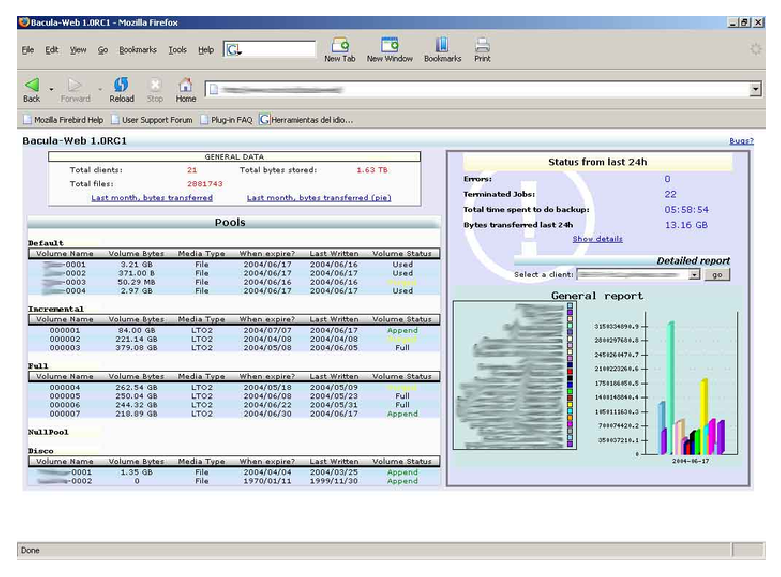
\includegraphics{./bweb-index.eps} \\
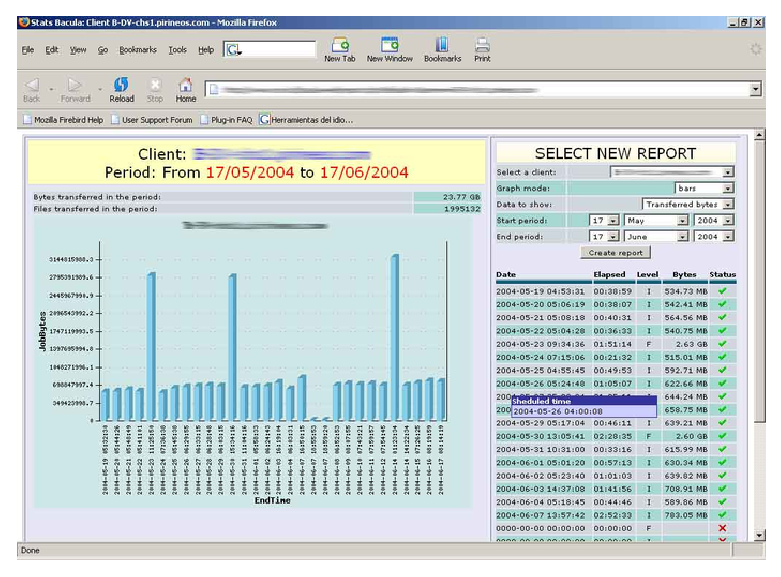
\includegraphics{./bweb-report.eps} \\

 

\section*{Notes}
\index[general]{Notes}
\addcontentsline{toc}{section}{Notes}
The output from bacula-web is best viewed with a resolution of
1024x768 or better. Most browsers will produce good results including 
MS Internet Explorer.

If you have configured bacula-web for a language other than English,
and the language changes are not being correctly displayed, restart
your web server.

\section*{Bugs}
\index[general]{Bugs}
\addcontentsline{toc}{section}{Bugs}

\begin{itemize}
\item In the Pie graphs, the margins don't work. It is a phplot bug.
\item The total elapsed time "calculation" is rudimentary.  If you have 2
or more concurrent jobs this is not real.
\end{itemize}

Submit your bugs at this link: 
\elink{http://indpnday.com/bacula_stuff/bacula-web/mantisbt/login_page.php}
{http://indpnday.com/bacula_stuff/bacula-web/mantisbt/login_page.php}.


\section*{Translations}
\index[general]{Translations}
\addcontentsline{toc}{section}{Translations}
If you want add a new language not supported by bacula-web please, follow
the following instructions:

Extract strings with this command (tsmarty2c.php is with bacula-web 
package):\\

\begin{verbatim}
./tsmarty2c.php templates > lang.c
xgettext lang.c
\end{verbatim}

Now you must have this file: messages.po \\
Edit messages.po to have your translations, then
send us a copy of the file.\\
